\documentclass[11pt,table]{article}

\usepackage{subfiles}
\usepackage[breakable]{tcolorbox}
%\usepackage{parskip} 

\usepackage{iftex}
\ifPDFTeX
\usepackage[T1]{fontenc}
\usepackage{mathpazo}
\else
\usepackage{fontspec}
\fi
\usepackage[english]{babel}
\usepackage{lipsum}
\usepackage{microtype}
\usepackage{float}
\usepackage{caption}


\usepackage{subcaption}
\usepackage[skip=50pt]{caption} % default 10pt
\captionsetup[figure]{skip=10pt}
\usepackage{rotating}
\usepackage{wrapfig}

\usepackage{graphicx}
\graphicspath{
  {figures/}
}  

\captionsetup{format=plain,
	aboveskip=-0.2cm,
	indention=0cm, 
	textformat=simple,
	textfont=small,
	labelfont=small, 
	justification=centering,
	labelfont=bf}



\usepackage[Export]{adjustbox} % Used to constrain images to a maximum size
\adjustboxset{max size={0.9\linewidth}{0.9\paperheight}}
\usepackage{float}
%\floatplacement{figure}{H} % forces figures to be placed at the correct location
\usepackage{xcolor}    % Allow colors to be defined
\usepackage{enumerate} % Needed for markdown enumerations to work
\usepackage{geometry}  % Used to adjust the document margins
\usepackage{amsmath}   % math symbols
\usepackage{amssymb}   % more math symbols
\usepackage{siunitx}   % write numbers and units nicely
% \usepackage{textcomp}  % defines textquotesingle
\usepackage[           % Literaturverwaltung mit BibLaTeX
  style=ieee,
  sorting=none
]{biblatex}                     
\addbibresource{bibliography.bib} % Pfad Literaturverzeichnis
\usepackage[autostyle=true]{csquotes} % Für BibLaTeX notwendig
\usepackage{upquote}   % Upright quotes for verbatim code
\usepackage{eurosym}   % defines \euro
% \usepackage[mathletters]{ucs} % Extended unicode (utf-8) support
\usepackage{fancyvrb}  % verbatim replacement that allows latex
\usepackage{grffile}   % extends the file name processing of package graphics 
% to support a larger range
\makeatletter % fix for grffile with XeLaTeX
\def\Gread@@xetex#1{%
	\IfFileExists{"\Gin@base".bb}%
	{\Gread@eps{\Gin@base.bb}}%
	{\Gread@@xetex@aux#1}%
}
\makeatother

\usepackage{hyperref}
\usepackage[capitalise]{cleveref}
\Crefname{figure}{Fig.}{Figs.}% {<type>}{<singular>}{<plural>}
\usepackage{acro}

% The default LaTeX title has an obnoxious amount of whitespace. By default,
% titling removes some of it. It also provides customization options.
\usepackage{titling}
\usepackage{longtable} 
\usepackage{booktabs}  
\renewcommand{\arraystretch}{1.2} % more space between table rows

\usepackage[inline]{enumitem}
\usepackage[normalem]{ulem}
% normalem makes italics be italics, not underlines
\usepackage{mathrsfs}

\captionsetup[table]{skip=10pt}


% Colors for the hyperref package
\definecolor{urlcolor}{rgb}{0,.145,.698}
\definecolor{linkcolor}{rgb}{0,0,0}%{.71,0.21,0.01}
\definecolor{citecolor}{rgb}{0,0,0}%{.12,.54,.11}


\title{Predicting Renewable Energy Production Using Machine Learning Methods}
\author{Luis Gentner, Leon Sengün, Dilara Yildiz}
\date{\today}



% Prevent overflowing lines due to hard-to-break entities
\sloppy 

\hypersetup{
	breaklinks=true,  % so long urls are correctly broken across lines
	colorlinks=true,
	urlcolor=urlcolor,
	linkcolor=linkcolor,
	citecolor=citecolor,
}
% Slightly bigger margins than the latex defaults

\geometry{verbose,tmargin=1in,bmargin=1in,lmargin=1in,rmargin=1in}

\newcommand{\ket}[1]{\left|{#1}\right\rangle}
\newcommand{\bra}[1]{\left\langle{#1}\right|}
\newcommand{\braket}[2]{\left\langle{#1}\middle|{#2}\right\rangle}



\usepackage{fancyhdr}
\addtolength{\headheight}{1.2cm} % make more space for the header
\pagestyle{fancy} %plain} % use fancy for all pages except chapter start
\fancyhead[L]{\leftmark}
%\lhead{\includegraphics[height=1.3cm]{logo2}} % left logo
\rhead{
\includegraphics[height=0.6cm]{header.png}}   % right logo
%\renewcommand{\headrulewidth}{0pt} % remove rule below header


\title{Project Title}
\author{Your Names}
\date{\today}



\begin{document}
\begin{titlepage} 
	\centering 
	\rule{\textwidth}{1pt} 
	\vspace{2pt}\vspace{-\baselineskip} 
	\rule{\textwidth}{0.4pt} 
	\vspace{0.1\textheight} 
	
	
	%%% Adjust your project title here
	{\Huge VERY LONG AND IMPRESSIVE TITLES}\\[0.5\baselineskip] 
	{\Large WITH}\\[0.5\baselineskip] 
	{\Huge SEVERAL LINES} 
	
	
	\vspace{0.025\textheight} 
	\rule{0.3\textwidth}{0.4pt} 
	\vspace{0.1\textheight}
	
	%%% Your names, if long, a "\\" in between may help to make things look better
	{\Large \textsc{First Name, Second Name, Et Cetera}} 
	
	\vfill 
	
	%%% You can include a nice image from your project here
	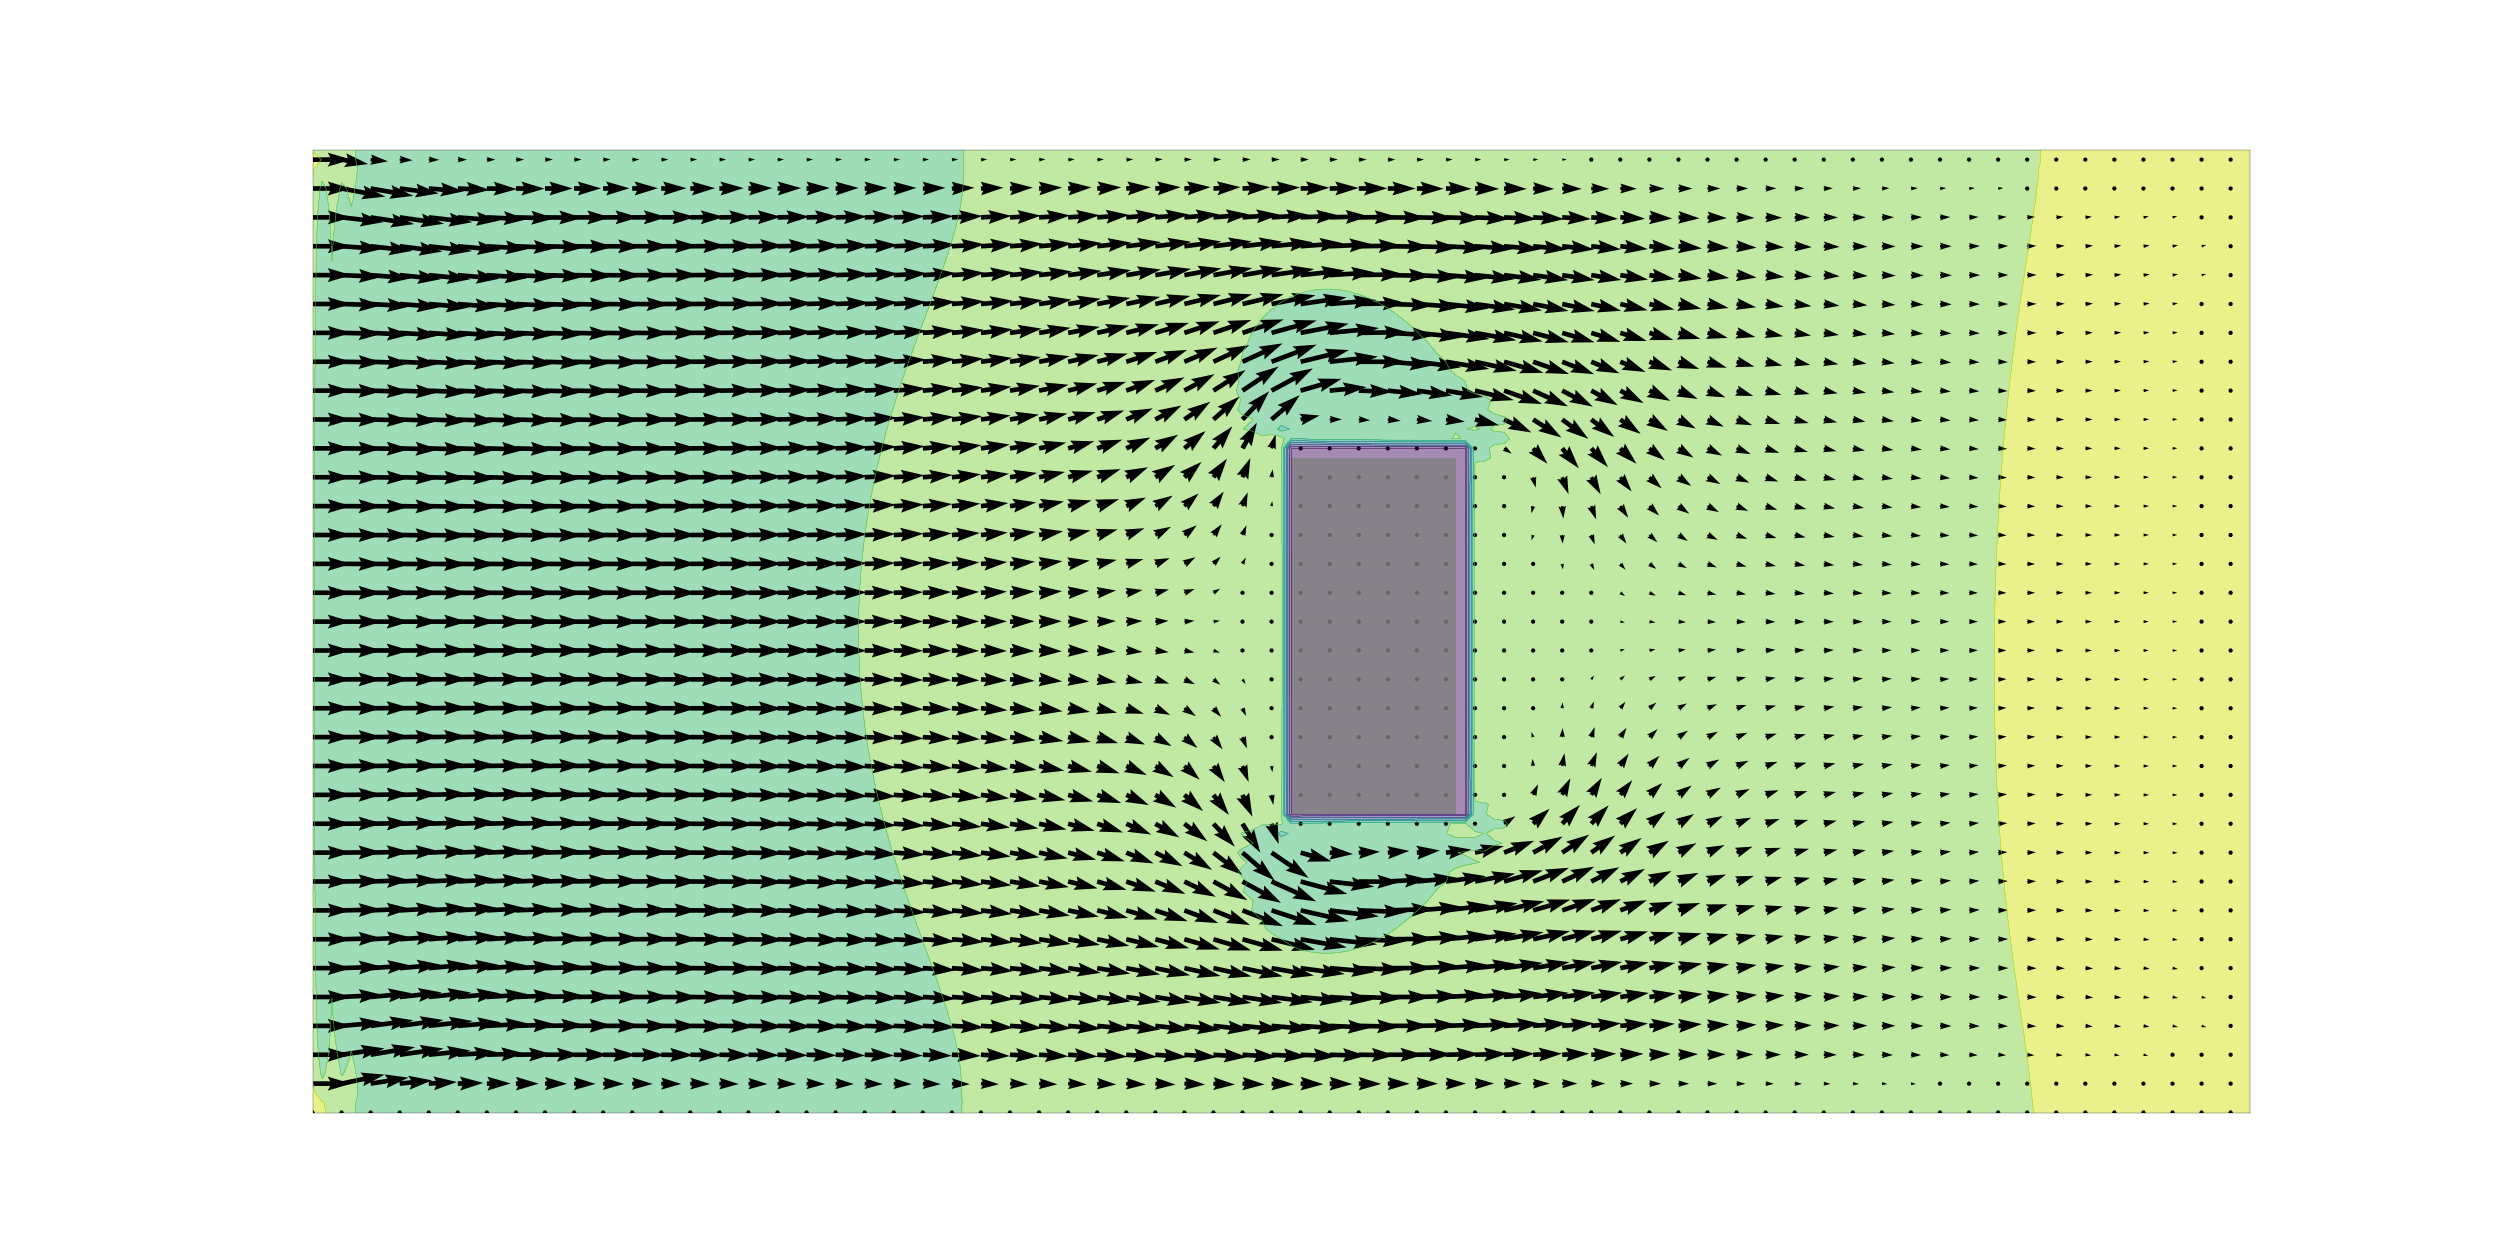
\includegraphics[width=0.5\linewidth]{Figures/example_cover.png} \\
	\vspace{0.05\textheight}
	{\large\textsc{Machine Learning Methods in Mechanics \\Report}\\ -\\ University of Stuttgart} 
	
	
	\vspace{0.1\textheight} 
	
	%%% Adjust the date here if you like
	{\normalsize \today}
	
	
	\rule{\textwidth}{0.4pt}
	\vspace{2pt}\vspace{-\baselineskip}
	\rule{\textwidth}{1pt}
	
\end{titlepage}

\pagenumbering{roman}

\newpage

\tableofcontents

\newpage

\pagenumbering{arabic}

%%% The following structure is a suggestion
%%% If you prefer to use your own, you can change everything
\section{Introduction}

Description of the project. Images are always a plus. You should reference each figure in the text and explain what can be seen. The flow field in Figure~\ref{fig:flow} shows particle velocities. It is taken from~\cite{Author2020}. What is the problem? What is the goal? What is your idea?\\ 

\begin{figure}[h]
	\centering
	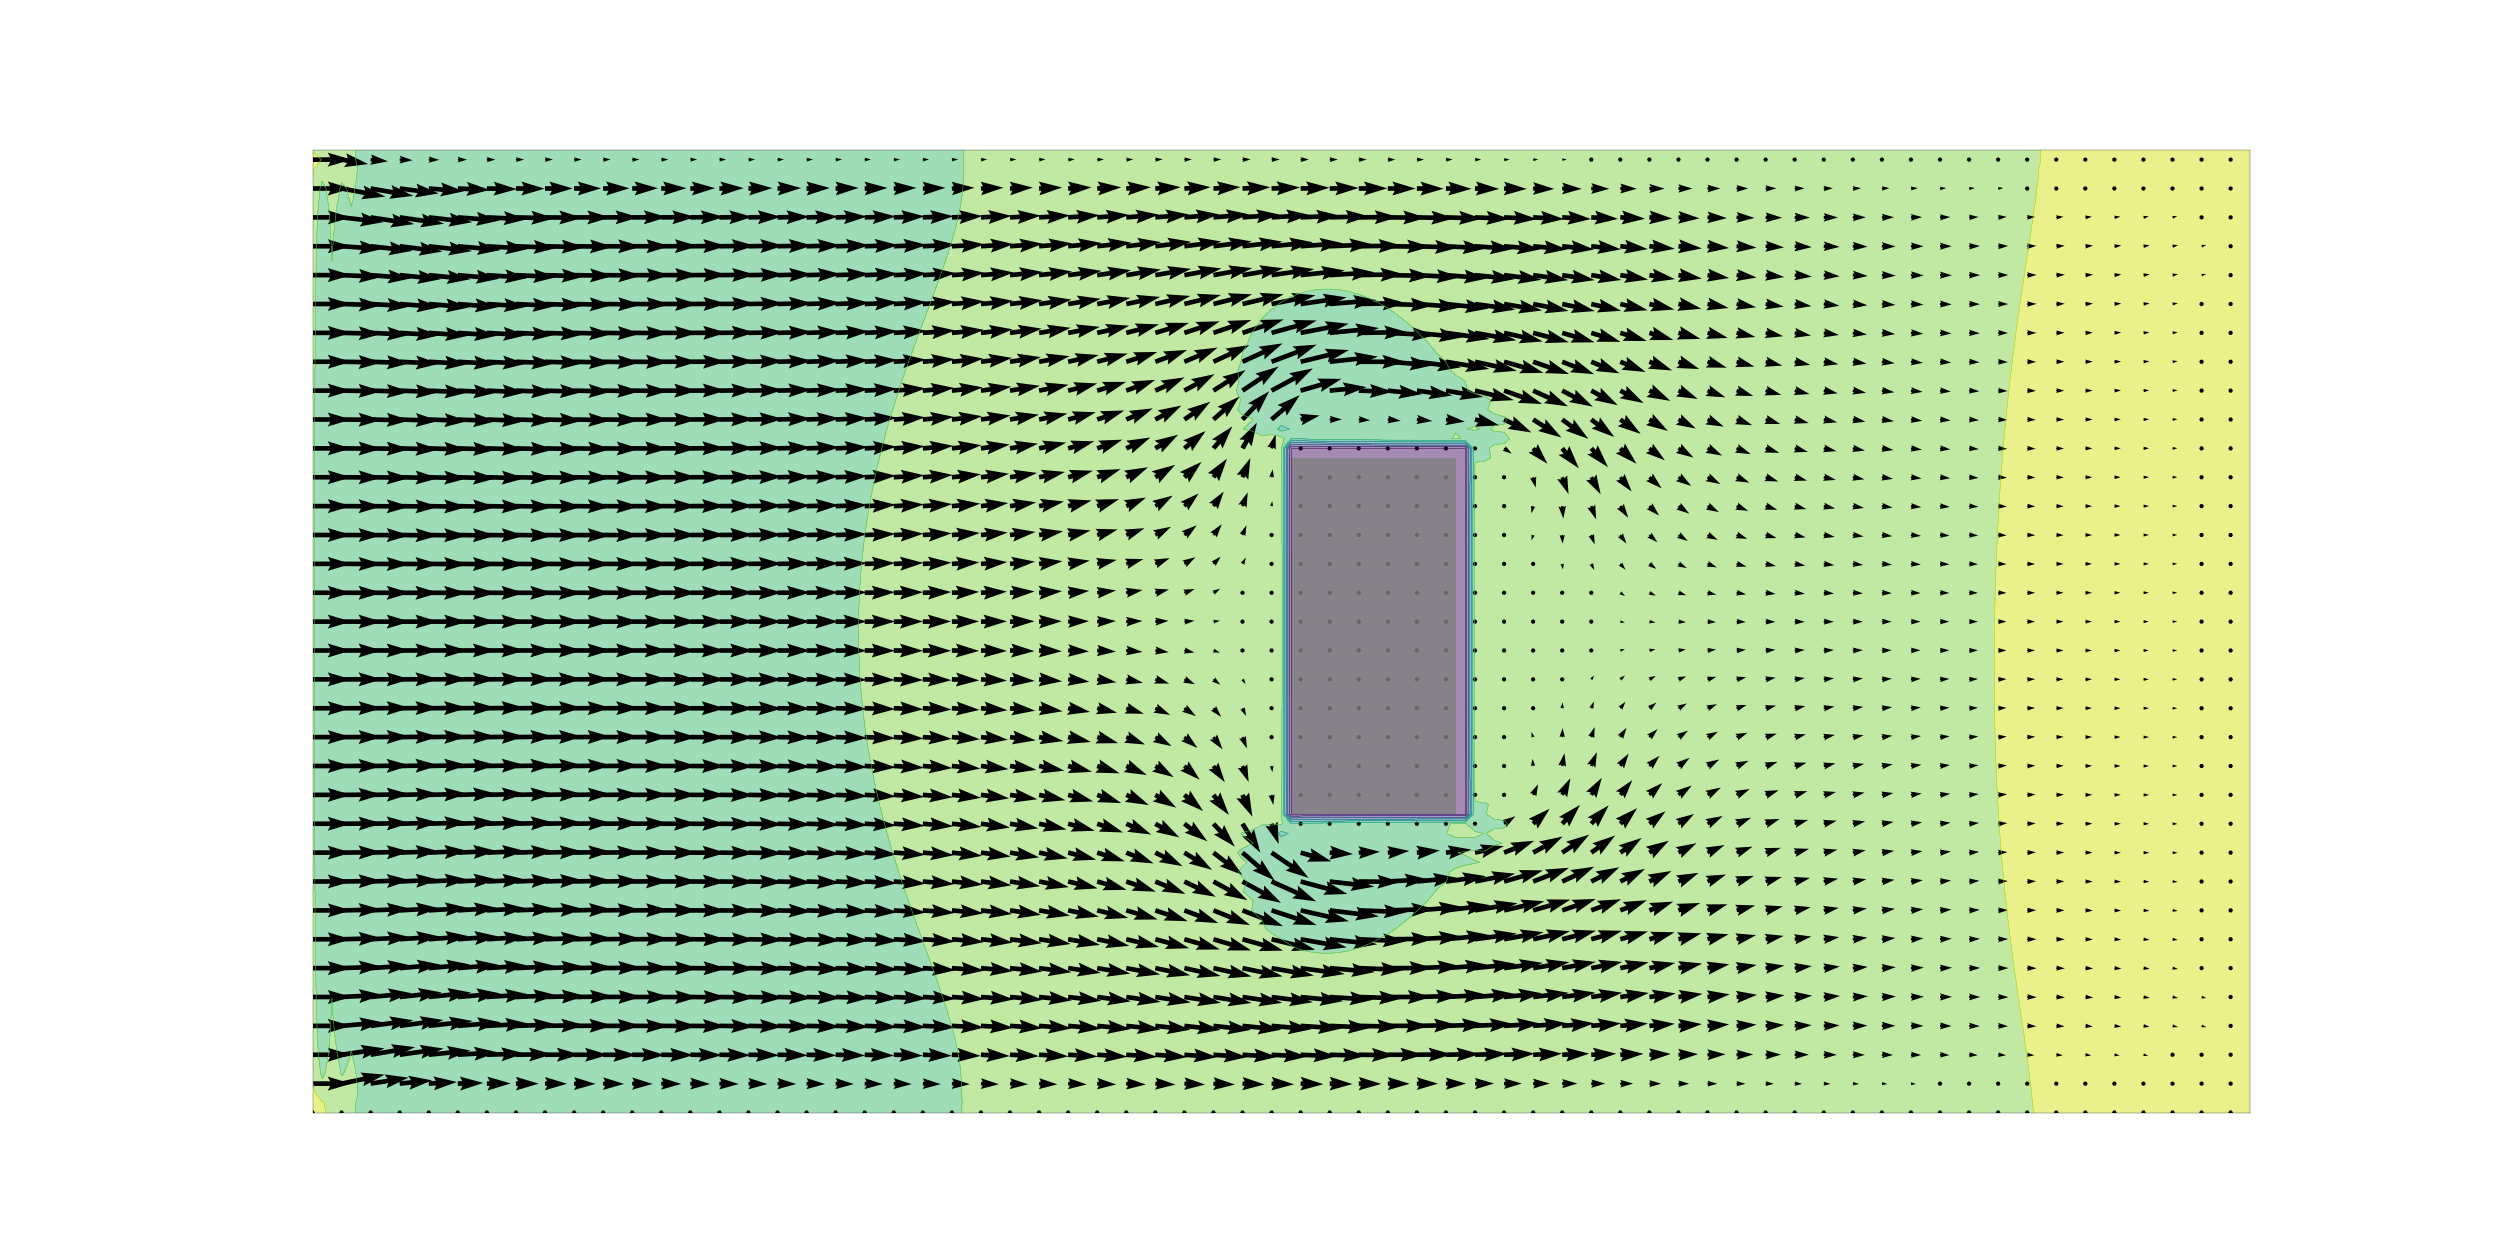
\includegraphics[scale=0.9]{Figures/example_cover.png}
	\caption{Flow field around a rectangular obstacle.}
	\label{fig:flow}
\end{figure}

%\lipsum[2]

You can include wrapped figures and tables, like Table~\ref{tab:features}. To make it work, there should be no newlines between the wrapped table or figure and the surrounding text. Normal tables work just as usual, like in Table~\ref{tab:other_parameters}.\\
\lipsum[1]

\begin{wraptable}{r}{0.55\textwidth}
	%\begin{table}[]
	%\centering
	%\vspace{0pt}
	\begin{tabular}{@{} lrrrrrr @{}}
		\toprule
		 & $L$ & $\lambda^S$ & $\mu^S$ & $k_{0\text{S}}^{\text{F}1}$ & $k_{0\text{S}}^{\text{F}2}$ & $k_{0\text{S}}^{\text{F}3}$ \\
		\midrule
		min & 0.6 & 3.1 & 15.8 & 0.1 & 0.003 & 0.1 \\
		max & 8.3 & 196.8 & 285.5 & 1.0 & 0.1 & 0.9 \\
		example & 1.33 & 21 & 126 & 0.18 & 0.05 & 0.23 \\
		\bottomrule
	\end{tabular}
	\caption{Feature values used for training the CNN.}\label{tab:features}
\end{wraptable} 

\lipsum[2-3]


\begin{table}[]
	\centering
	%\vspace{0pt}
	\begin{tabular}{@{} lrrrrrr @{}} 
		\toprule
		 & $L$ & $\lambda^S$ & $\mu^S$ & $k_{0\text{S}}^{\text{F}1}$ & $k_{0\text{S}}^{\text{F}2}$ & $k_{0\text{S}}^{\text{F}3}$ \\
		\midrule
		min & 0.6 & 3.1 & 15.8 & 0.1 & 0.003 & 0.1 \\
		max & 8.3 & 196.8 & 285.5 & 1.0 & 0.1 & 0.9 \\
		example & 1.33 & 21 & 126 & 0.18 & 0.05 & 0.23 \\
		\bottomrule
	\end{tabular}
	\caption{Values used to create the simulation in Figure~\ref{fig:flow}.}\label{tab:other_parameters}
\end{table}


\section{Computational Fluid Dynamics}

\subsection{The Navier-Stokes-Equations}

Equations as usual, like in Equation~\ref{equ:max_entropy}. Recall that equations like

\begin{equation}\label{equ:max_entropy}
	\phi_\mathrm{max} = \max_{\theta} \left[ \log(\sin(\theta - \exp(\theta))) - \theta^2 \right]
\end{equation}

are part of the text and should be treated like a word.

\lipsum[1]

Or without numbering, like the realtivistic kinetic energy 

\begin{equation*}
	E = \frac{mc^2}{\sqrt{1 - \frac{v^2}{c^2}}},
\end{equation*}

which yields the Newtonian kinetic energy $E = \frac 1 2 m v^2$ when linearized for small velocities $v$.

\subsection{Solution Method}
\lipsum[3-4]
\begin{wrapfigure}{r}{0.55\textwidth}
	\centering
	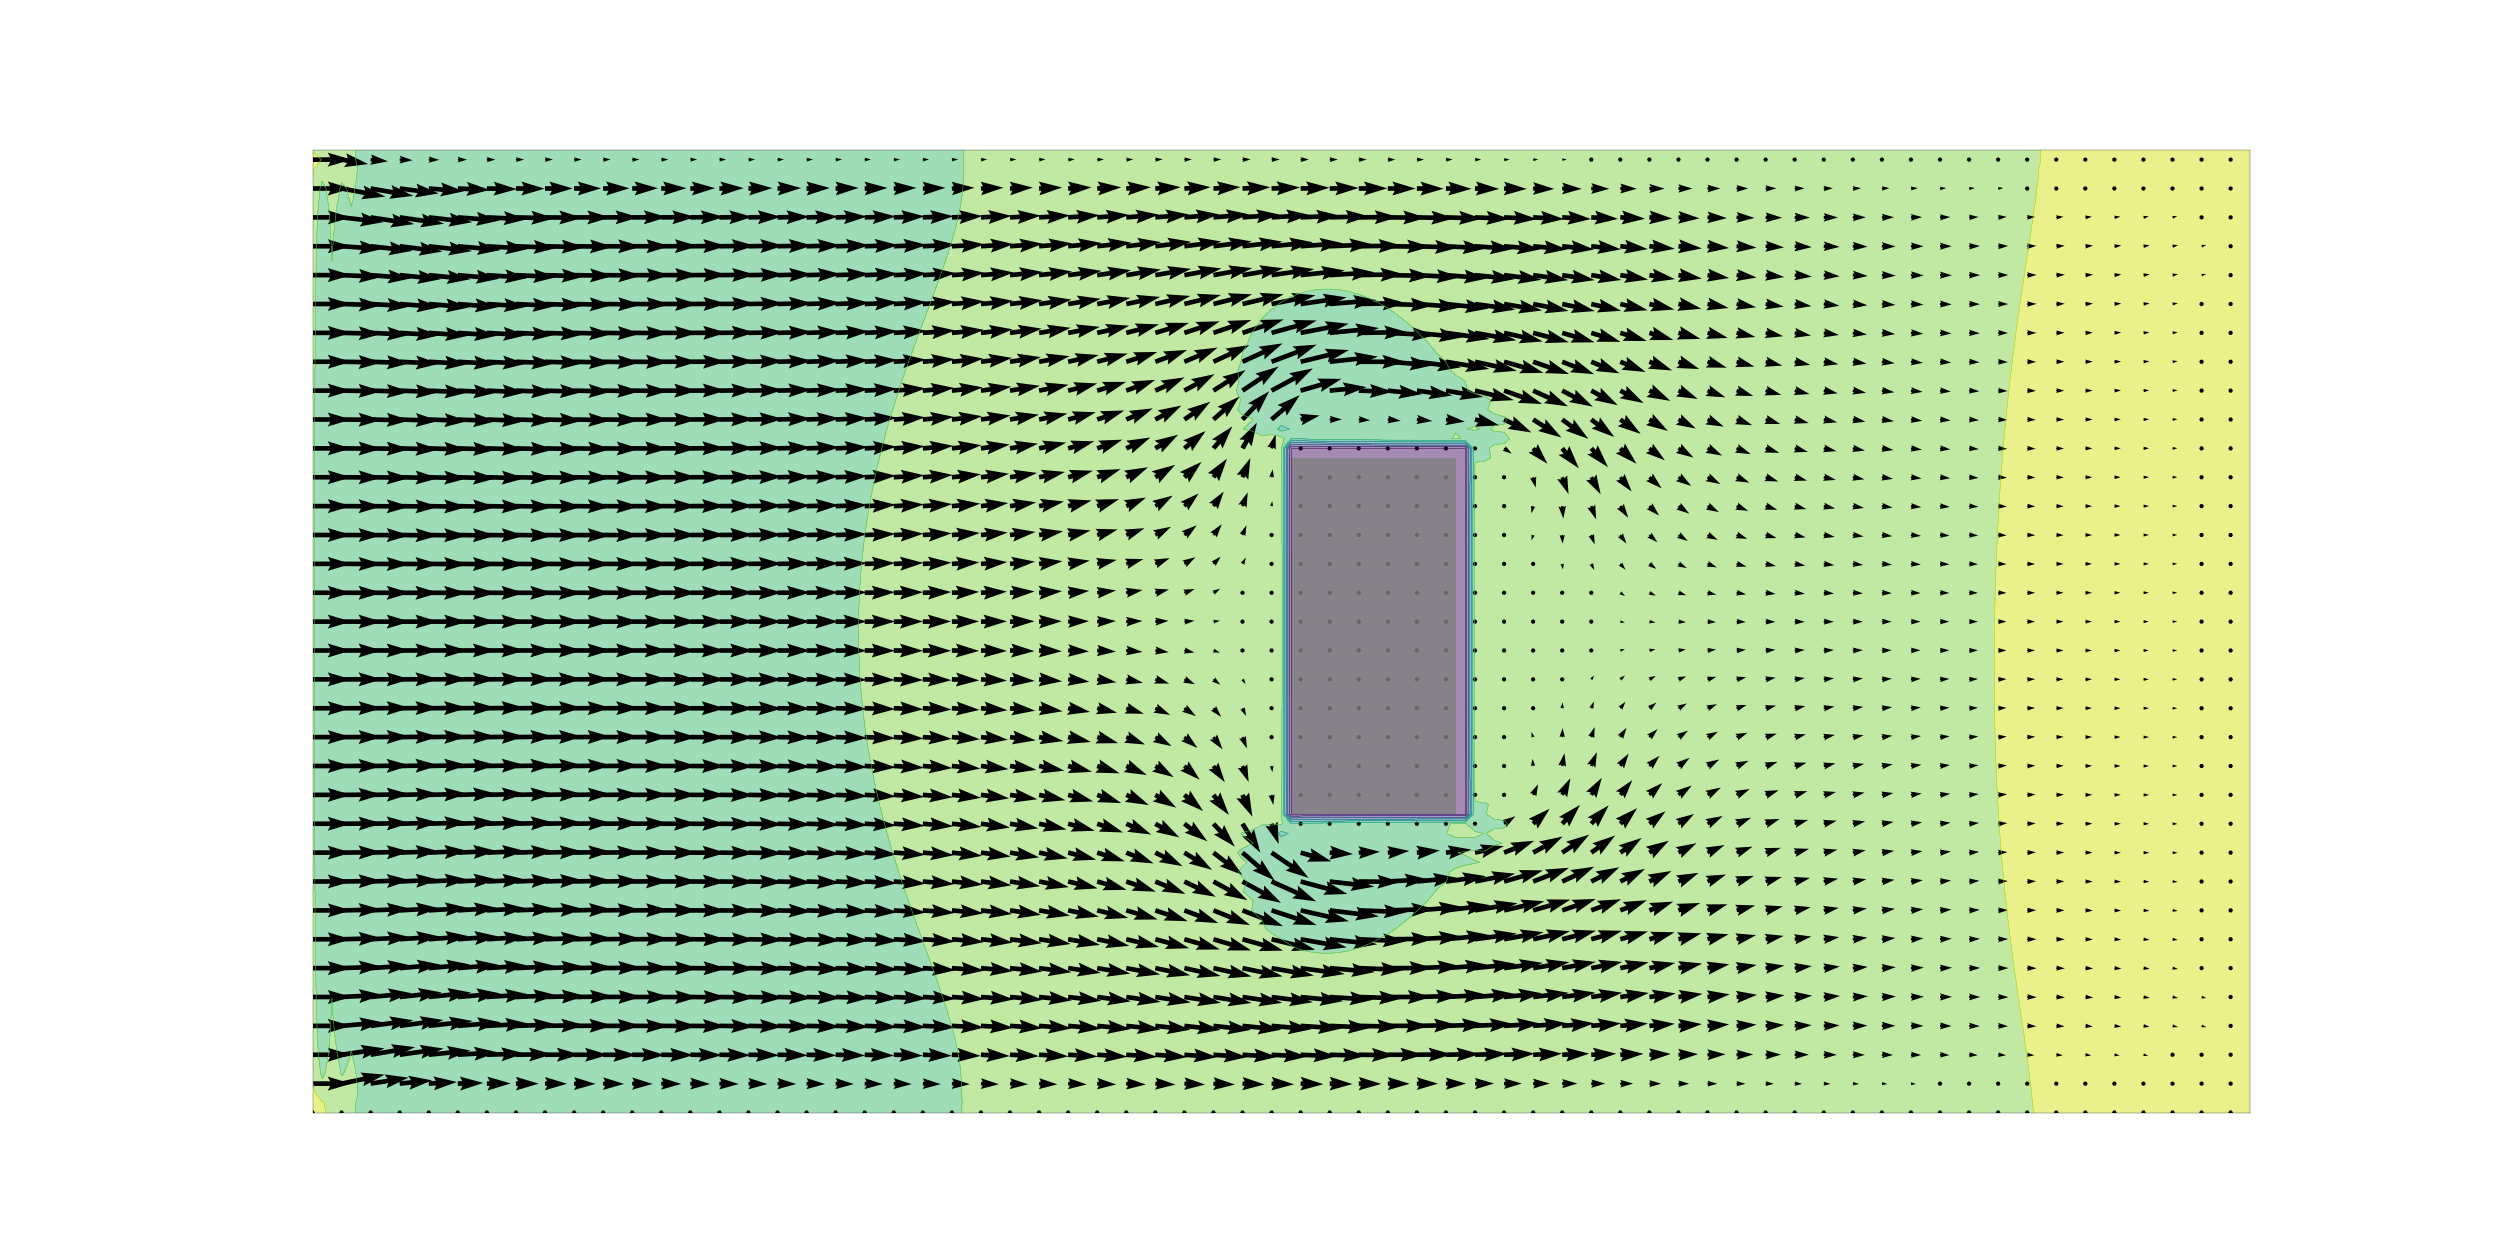
\includegraphics[scale=1.0]{Figures/example_cover.png}
	\caption{You can also use wrapped figures like this.}
	\label{fig:wrapfigure_example}
\end{wrapfigure}
\lipsum[5] \\ \newline
Figure~\ref{fig:wrapfigure_example} shows how to include wrapped figures that text can float around. Depending on what is depicted and how large it is, it may look better than a full figure.

\section{Convolutional Neural Networks}

\lipsum

\section{Idea and Data Generation}

\lipsum

\section{Results}

\lipsum

\begin{footnotesize}
\bibliographystyle{acm}


%%% This builds the bibliography
%%% You can use either bibtex with the following line and the "bibliography.bib" file
%%% OR ALTERNATIVELY comment the next line and uncomment the "thebibliography" environment

\bibliography{bibliography}

%%% comment the line above and uncomment the lines below
%%% for manually creating the bibliography

%\begin{thebibliography}{1}
%	
%	\bibitem{Author2020}% 
%	\textsc{A.\,W.~Harrow, A.~Hassidim, and S.~Lloyd},
%	\emph{Physical review letters 113} (15), 150502, (2009)
%	
%	\bibitem{Author2012}% 
%	\textsc{A.\,Y.~Kitaev},
%	\emph{Russian Mathematical Surveys 52} (6) p.\,1191--1249, (1997)
%	
%	
%\end{thebibliography}


\end{footnotesize}


%\newpage

\end{document}